\documentclass[12pt]{article}

\usepackage{epsfig}
\usepackage{amsmath}

\begin{document}
\noindent Luke Palmer  \\
          September 7, 2004 Physics 1120

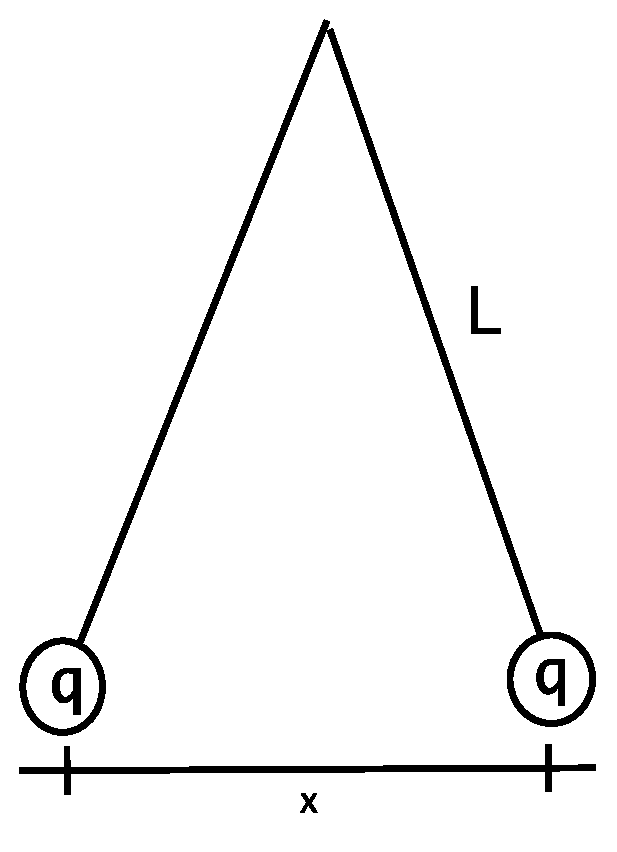
\epsfig{file=hw.eps,height=3in}

This is an easy problem once you get the measurements set up
conveniently.  First let's find out what $\theta$ is:

\[  \sin{\theta} = \frac{x}{2L} \]

Which means gravity must be pulling inward on each of the blocks with
force $F_g$:

\[  F_g = mg \sin{\theta} = \frac{mgx}{2L} \]

(No approximation necessary!)

And that means that the electric force is precisely that:

\[  F_e = \frac{mgx}{2L} = \frac{q^2}{4\pi\epsilon{}_0x^2} \]

Finding the solution is trivial:

\[  q = \sqrt{\frac{2\pi\epsilon{}_0 mgx^3}{L}} \]

For the second part, if I were to put ten million electrons on each
ball, the charge on each would be:

\[  q = 10^7e = 1.602 \times 10^{-12} \, C \]

Making the force between them:

\[  F = \frac{q^2}{4\pi\epsilon{}_0 r^2} = 2.307 \times 10^{-10} \, N \]

For a reasonable $r$ ($1 \, \mathit{cm}$).  In other words, it would be
entirely unnoticable unless the ping pong balls were \textit{extremely}
light, something like a thousand times as light as a paperclip.  I know
of no such ping pong ball.

\end{document}
